\printconcepts

\exercise{What is the name of the rule which states that $\ds \frac{d}{dx}\big(x^n\big) = nx^{n-1}$, where $n>0$ is an integer?}{Power Rule.}

\exercise{What is $\ds \frac{d}{dx}\big(\ln x\big)$?}{$1/x$}

\exercise{Give an example of a function $f(x)$ where $\fp(x) = f(x)$.}{One answer is $f(x) = 10e^x$.}

\exercise{Give an example of a function $f(x)$ where $\fp(x) = 0$.}{One answer is $f(x) = 10$.}

\exercise{The derivative rules introduced in this section explain how to compute the derivative of which of the following functions?

\noindent\begin{minipage}[t]{.5\linewidth}
\begin{itemize}
\item	$\ds f(x) = \frac{3}{x^2}$ 
\item	$g(x) = 3x^2-x+17$ 
\item	$h(x) = 5\ln x$ 
\end{itemize}
\end{minipage}%
\begin{minipage}[t]{.5\linewidth}
\begin{itemize}
\item	$j(x) = \sin x \cos x$ 
\item		$k(x) = e^{x^2}$
\item	$m(x) = \sqrt{x}$
\end{itemize}
\end{minipage}
}{$f(x)$, $g(x)$, $h(x)$, and $m(x)$}

\exercise{Explain in your own words how to find the third derivative of a function $f(x)$.}{Answers will vary.}

\exercise{Give an example of a function where $\fp(x) \neq 0$ and $\fpp(x) = 0$.}{One possible answer is $f(x) = 17x-205$.}

\exercise{Explain in  your own words what the second derivative ``means.''}{Answers will vary.}

\exercise{If $f(x)$ describes a position function, then $\fp(x)$ describes what kind of function? What kind of function is $\fpp(x)$?}{$\fp(x)$ is a velocity function, and $\fpp(x)$ is acceleration.}

\exercise{Let $f(x)$ be a function measured in pounds, where $x$ is measured in feet. What are the units of $\fpp(x)$?}{lbs/ft$^2$.}

\printproblems

\input{exercises/02_03_exset_01}

\exercise{A property of logarithms is that $\ds \log_a x = \frac{\log_b x}{\log_b a}$, for all bases $a,b>0$ and $a,b\neq 1$.
\begin{enumerate}
	\item Rewrite this identity when $b=e$, i.e., using $\log_ex =\ln x$.
	\item	Use part (a) to find the derivative of $y=\log_a x$. 
	\item	Give the derivative of $y=\log_{10} x$.
\end{enumerate}}{}

\exercise{Prove the Constant Rule: $\dfrac {d}{dx} (c)=0$, where $c$ is constant.}{$\displaystyle\frac {d}{dx}(c) = \lim_{h\to 0} \frac{c - c}{h}=\lim_{h\to 0}0=0$}

\exercise{The figure shows the graphs of $f$, $\fp$, and $\fpp$. Identify each curve and explain your choices.\\
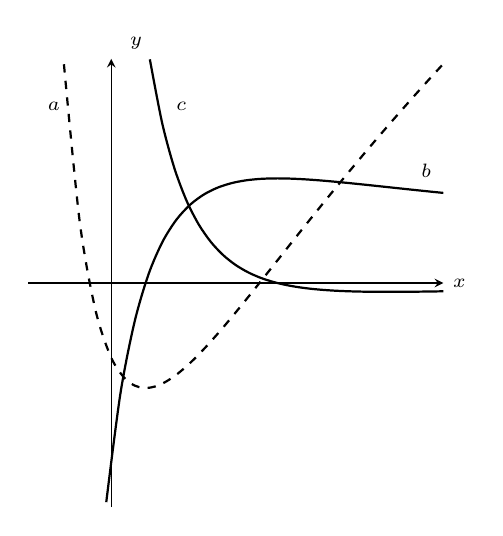
\begin{tikzpicture}
 \begin{axis}[xtick=\empty, ytick=\empty, axis y line=middle,axis x line=middle,
   ymin=-3,ymax=3, xmin=-1,xmax=4, name=myplot, xscale=1/1.3,]
  \addplot [draw={\colorone}, dashed, smooth, domain=-.57:4,thick]
   {(6*(x*x*x-4*x)/((x+2)*(x+2)*(x+2)) +.65*x-1}; % Curve a
  \node[label={30:{\scriptsize $a$}}] at (axis cs:-1,2.1) {};
  \addplot [draw={\colortwo}, smooth, domain=-.06:4,thick]
   {(13*x*x*x+78*x*x+876*x-376)/(20*x*x*x+120*x*x+240*x+160)}; %Curve b
  \node[label={30:{\scriptsize $c$}}] at (axis cs:.55,2.1) {};
  \addplot [draw={\colorone}, smooth, domain=.465:4, thick]
   {(-72*x+144)/(x*x*x*x+8*x*x*x+24*x*x+32*x+16)}; %Curve c
  \node[label={30:{\scriptsize $b$}}] at (axis cs:3.5,1.2) {};
 \end{axis}
 \node [right] at (myplot.right of origin) {\scriptsize $x$};
 \node [above] at (myplot.above origin) {\scriptsize $y$};
\end{tikzpicture}}{$a$ is $f$, $b$ is $\fp$, $c$ is $\fpp$}

\exercise{The figure shows the graphs of $f$, $\fp$, $\fpp$ and $\fpp'$. Identify each curve and explain your choices.\\
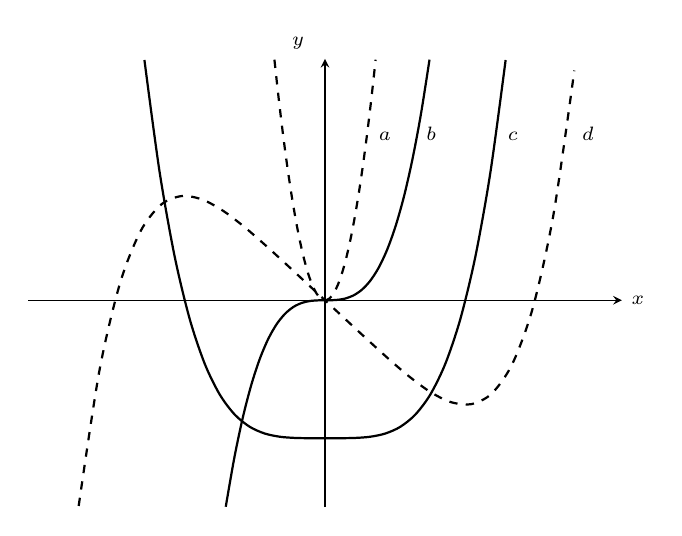
\begin{tikzpicture}
 \begin{axis}[xtick=\empty, ytick=\empty, axis y line=middle,axis x line=middle,
   ymin=-3,ymax=3.5, xmin=-2,xmax=2, name=myplot, xscale=1.1/1,]

  \addplot [draw={\colorone}, dashed, smooth, domain=-1.66:1.68,thick] {.5*x*x*x*x*x-2*x}; 
  \node[label={30:{\scriptsize $d$}}] at (axis cs:1.6,2.1) {};

  \addplot [draw={\colortwo}, smooth, domain=-1.217:1.217,thick] {2.5*x*x*x*x-2};
  \node[label={30:{\scriptsize $c$}}] at (axis cs:1.1,2.1) {};

  \addplot [draw={\colorone}, smooth, domain=-.669:.704, thick] {10*x*x*x};
  \node[label={30:{\scriptsize $b$}}] at (axis cs:.55,2.1) {};

  \addplot [draw={\colortwo}, dashed, smooth, domain=-.341:.341, thick] {30*x*x};
  \node[label={30:{\scriptsize $a$}}] at (axis cs:.23,2.1) {};

 \end{axis}
 \node [right] at (myplot.right of origin) {\scriptsize $x$};
 \node [above] at (myplot.above origin) {\scriptsize $y$};
\end{tikzpicture}}{$d$ is $f$, $c$ is $\fp$, $b$ is $\fpp$, and $a$ is $\fpp'$}

\input{exercises/02_03_exset_02}

\exercise{The position of a object is described by $s(t)=t^4 - 4t^2$, $t \geq 0$, where $s$ is in feet and $t$ is in seconds. Find
\begin{enumerate}
\item the velocity and acceleration functions for the object,
\item the acceleration after 1.5 seconds, and
\item the time(s), in seconds, when the object is at rest.
\end{enumerate}}{\mbox{}\\[-2\baselineskip]\begin{enumerate}
\item $v(t) = 4t^3 - 8t$, $a(t)=12t^2 - 8$
\item $a(1.5) = 19\ \text{ft/s}^2$
\item $t=0$ sec and $t=\sqrt2$ sec
\end{enumerate}}

\exercise{The position of a object is described by $s(t)=5e^t-5t$, where $s$ is in inches and $t$ is in seconds. Find
\begin{enumerate}
\item the velocity and acceleration functions for the object,
\item the acceleration after 2 seconds, and
\item the acceleration when the object is at rest.
\end{enumerate}}{\mbox{}\\[-2\baselineskip]\begin{enumerate}
\item $v(t) = 5e^x-5$, $a(t)=5e^x$
\item $a(2) = 5e^2\ \text{ft/s}^2$
\item $v(t)=0$ at $t=0$ sec, $a(0)=5\ \text{in/s}^2$ 
\end{enumerate}}

\questioncolumnbreak

\exerciseset{In Exercises}{, find the equations of the tangent line %and normal lines
to the graph of the function at the given point.
}{

\exercise{$f(x)=x^3-x$ at $x=1$
}{Tangent line: $y = 2(x-1)$
%
%Normal line: $y=-1/2(x-1)$
}

\exercise{$f(t)=e^t+3$ at $t=0$
}{Tangent line: $y = t+4$
%
%Normal line: $y=-t+4$
}

\exercise{$g(x)=\ln x$ at $x=1$
}{Tangent line: $y = x-1$
%
%Normal line: $y=-x+1$
}

\exercise{$f(x)=4\sin x$ at $x=\pi/2$
}{Tangent line: $y = 4$
%
%Normal line: $x=\pi/2$
}

\exercise{$f(x)=-2\cos x$ at $x=\pi/4$
}{Tangent line: $y = \sqrt{2}(x-\frac{\pi}{4})-\sqrt{2}$
%
%Normal line: $y = \frac{-1}{\sqrt{2}}(x-\frac{\pi}{4})-\sqrt{2}$
}

\exercise{$f(x)=2x+3$ at $x=5$
}{Tangent line: $y = 2x+3$
%
%Normal line: $y=-1/2(x-5)+13$
}

}

\exercise{Find the two values of $n$ so that the function $y=x^n$ satisfies the differential equation $x^2y\primeskip''+2xy\primeskip'-6y=0$.}{$n=-3,2$}

\printreview

\exercise{Given that $e^0=1$, approximate the value of $e^{0.1}$ using the tangent line to $f(x) = e^x$ at $x=0$.}{The tangent line to $f(x) = e^x$ at $x=0$ is $y=x+1$; thus $e^{0.1} \approx y(0.1) = 1.1$. }

\exercise{Approximate the value of $(3.01)^4$ using the tangent line to $f(x) = x^4$ at $x=3$.}{The tangent line to $f(x) = x^4$ at $x=3$ is $y=108(x-3)+81$; thus $(3.01)^4 \approx y(3.01) = 108(.01)+81 = 82.08$. }
